
\section{Introduction}

%%** Introducing codon models and their usefulness **
Phylogenetic codon models are now routinely used in many domains of bioinformatics and molecular evolutionary studies.
Most often used to characterize the selective regimes, or genes, or sites, having experienced positive selection.
More generally, these models highlight the respective contributions of mutation, selection, genetic drift and biased gene conversion, and the causes of their variation between genes or across species.

%** introducing the idea of a single $\omega$ **
Conceptually, codon models take advantage of the fact that synonymous and non-synonymous substitutions are differentially impacted by selection.
Assuming synonymous mutations are neutral, the synonymous substitution rate equal to the underlying mutation rate.
Non-synonymous substitutions, on the other hand, reflect the combined effect of mutation and selection.
Classical codon models formalize this idea by invoking a single parameter $\omega$, acting multiplicatively on non-synonymous substitutions rates \citep{Muse1994, Goldman1994}.
Using a parametric model automatically corrects for the multiplicity issues created by the complex structure of the genetic code and by uneven mutation rates between nucleotides.
As a result, this parameter $\omega$ capture the net, or aggregate, effect of selection on non-synonymous mutations.

%** elaborating on the phenomenological versus mechanistic, classical versus mutsel, distinction **
Classical codon models, so defined, are phenomenological, they capture a complex mixture of selective effects through a single parameter.
In reality, the selective effects of associated with non-synonymous mutations depend on the context, and on the initial and final amino acids.
In contrast, attempts at an explicitly modelling of these complex selective landscapes have been formulated, named mechanistic codon models, based on the mutation-selection formalism \citep{Halpern1998}.
However, these models are computationally complex~\citep{Rodrigue2010, Tamuri2012}, and classical codon models therefore remain an attractive, potentially more robust, although still perfectible, approach.

%** bringing in the key issue here: correctly teasing apart mutation and selection **
This simple parametric design of current classical models raises an important question.
By capturing selection through a single parameter, $\omega$, is the mutational process estimated reliably?
There are indications that this is not the case.
In their simplest form \citep{Muse1994}, classical codon models predict that the nucleotide composition should be the same for all three positions of the codons, and should be equal to the nucleotide equilibrium frequencies implied by the underlying nucleotide substitution rate matrix.
In reality, composition differ, the third position shows more extreme composition, reflecting the underlying mutation bias, compared to first and second positions, which are typically closer to 50\% GC \citep{Singer2000}.

%** Ici, je pense qu’il faut un peu développer sur le formalisme 3x4, qui est directement pertinent **
These modulations across the three coding positions have been accommodated using the so-called 3x4 formalism, allowing for different nucleotide rate matrices at the three positions.
However, this is problematic, this modelling has the consequence that synonymous substitutions, say, from A to C, occur at different rates at the first and third positions.
Yet, in reality, the mutation process is blind to the coding structure, and should be homogeneous across coding positions, and if neutral, all mutations from A to C should have the same rate.
In any case: this suggests that the mutation matrix (F1x4) or matrices (F3x4) estimated by codon models are not correctly reflecting the mutation rates between nucleotides.
Instead, what these matrices are capturing is the result of the compromise between mutation and selection at the level of the realized nucleotide frequencies.

%** potential impact of these problems: both practical and conceptual **
For detecting selection, this problem is probably minor.
Conceptually, however, this is a clear symptom of a more fundamental problem, mutation rates and fixation probabilities are not correctly teased apart.
Practically, could have important consequences in other contexts than tests of positive selection.
In particular, there is a current interest in investigating the variation between species in GC content, and its effect on the evolution of protein-coding sequences.
A particularly important factor here is biased gene conversion toward GC (named gBGC), which can confound the tests for detecting positive selection~\citep{Galtier2009,Ratnakumar2010, Figuet2014}.
Even in the absence of gBGC, however, uneven mutation rates, varying across species, can have an important impact on the estimation of the strength of selection~\citep{Galtier2009,Ratnakumar2010, Figuet2014}.
All this suggests that, even before introducing gBGC in codon models, correctly formalizing the interplay between mutation and selection in current codon models would be an important thing to do.

%** the mut-sel balance revisited: an equilibrium between two net forces **
In this direction, the key point that needs to be correctly formalized is that the nucleotide's realized frequencies are the result of a compromise between mutation and selection, then this implies that the strength of selection is not the same between all nucleotide or amino-acid pairs.
For instance, if the mutation process is AT-biased, because of selection, the realized nucleotide frequencies at equilibrium will be less AT-biased than expected under the mutation process.
However, this implies that, at equilibrium, there will be a net mutation pressure toward AT, which has to be compensated for by a net selection differential toward GC, or, in other words, that mutations toward AT will be more deleterious on average than those toward GC.
As a result, the net $\dnds$ toward AT will be lower than the net $\dnds$ toward GC.

%** introducing $\omega$ as a tensor **
All this suggests that, in order for a codon model to correctly formalize this subtle interplay between mutation and selection, the component of the parameter vector responsible for absorbing the net effect of selection (i.e. $\omega$) should not be a scalar, as is currently the case.
Instead, it should be a tensor, an array of $\omega$ values unfolding along multiple directions.
However, how many components should this tensor contain?
More generally, what is the simplest parametric structure able to correctly tease apart mutation rates on one hand, and net mean fixation probabilities caused by selection, on the other hand, and this, without having to explicitly model the underlying fitness landscape?

%** end of introduction: outline of the mean-field approach and of the results — à compléter à la fin **
In the present work, we address these questions.
In order to derive a codon model along those lines, our strategy is to first assume a true site-specific evolutionary process, following the mutation-selection formalism.
Then, we derive the mean substitution process implied across all sites by this mechanistic model.
Inferring parameters on simulated alignments, we show that the model correctly estimates the mutation rates.

% Improved inference of site-specific positive selection under a generalized parametric codon model when there are multinucleotide mutations and multiple nonsynonymous rates~\citep{Dunn2019}.
% Influence of mutation bias and hydrophobicity on the substitution rates and sequence entropies of protein evolution~\citep{Santos2018}.

\section{Results}

We first conduct simulation experiments with a mutation-selection substitution model with fixed fitness landscape, based on two parameters tuning the mutation bias and the stringency of selection.
We explore, through summary statistics the intricate interplay between mutation and selection.
In a second step, we explore how codon models with alternative parameterization are able to capture the mutation and selection of the evolutionary process.

\subsection{Simulations experiments}

Simulations of protein-coding DNA sequences were conducted under an origin-fixation substitution process~\citep{McCandlish2014} at the level of codons, parameterized by two variables (see figure~\ref{fig-mut-bias:parameters}).
In this context, mutations are defined at the level of nucleotides with a single parameter controlling mutational bias toward AT $\lambda = (\mutequi_A+\mutequi_T)/(\mutequi_C+\mutequi_G)$, which is shared by all sites of the sequence (see section~\ref{sec-mut-bias:mut-matrix}).
With regards to selection, synonymous mutations are considered neutral, such that the synonymous substitution rate equal to the underlying mutation rate.
Alternatively, selection is modelled for non-synonymous mutations, with each codon site of the sequence defined by its own profile of amino-acid fitness (a vector of 20 fitnesses), drawn from a Dirichlet distribution of concentration parameter $\alpha$ (see section~\ref{sec-mut-bias:aa-selection}).
A low parameter $\alpha$ implies that the amino-acid profile randomly drawn is likely uneven, with some-acid with high fitness while other are with low fitness (for each site of the sequence).
Ultimately, the stringency of selection increase with decreasing $\alpha$.

\begin{figure}[H]
    \centering
    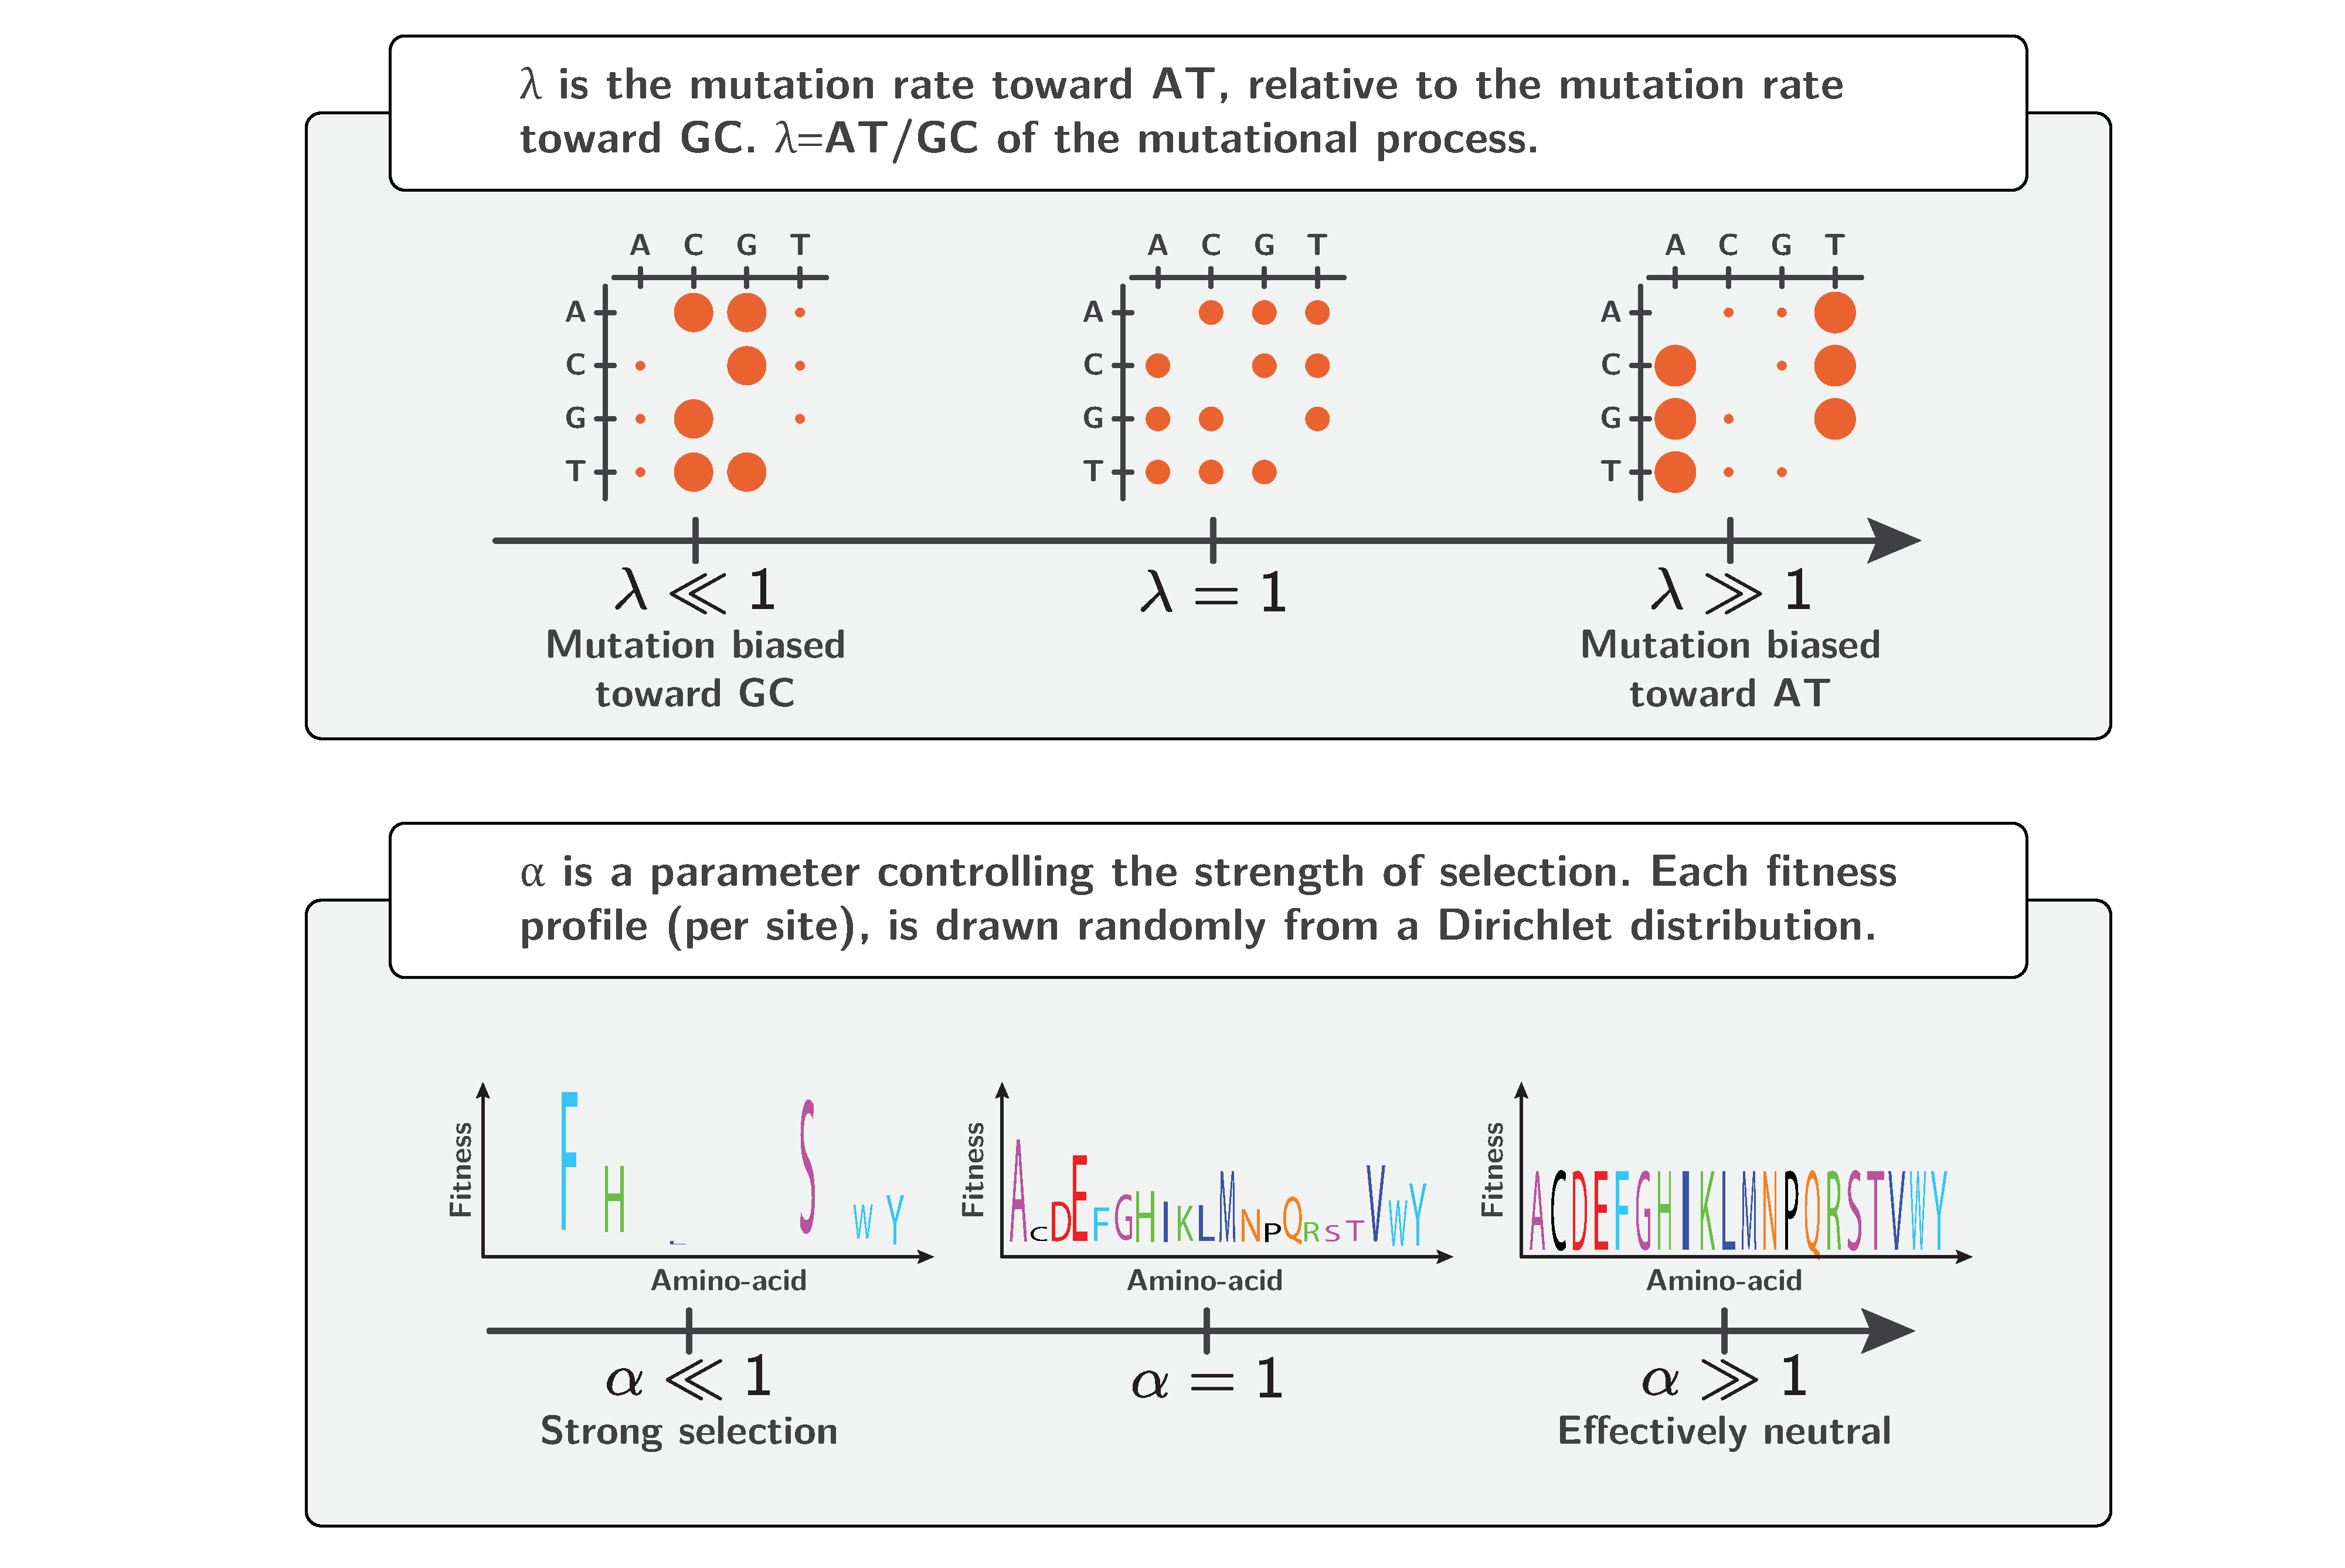
\includegraphics[width=\textwidth] {parameters}
    \caption[Parameters of the mutation-selection model]{
    Parameters of the mutation-selection model.
    Mutational bias (toward A and T) is shared by all sites of the sequence, and tuned by the parameter $\lambda$.
    Conversely, each site of the sequence is defined by a unique fitness profile, drawn from a Dirichlet distribution with concentration parameter $\alpha$.
    Stringency of selection increase with decreasing $\alpha$.}
    \label{fig-mut-bias:parameters}
\end{figure}

\subsubsection{Observed behaviour}

Simulation of this origin-fixation process along a species tree result in a multiple sequence alignment of DNA for the extant species (see section~\ref{sec-mut-bias:simu}), from which summary statistics can be computed.
One such straightforward summary statistic is the frequency of the different nucleotides, and the resulting observed mutational bias $\atgc$ of the alignment.
Such observed mutational bias is compared to underlying mutational bias $\lambda$ at different positions of the codon (first, second and third), as depicted in figure~\ref{fig-mut-bias:AT-GC-obs}).
The third position of codons reflects the mutational bias.
However the first and second positions are impacted by the strength of selection and display less extreme bias than the underlying mutational bias.

\begin{figure}[H]
    \centering
    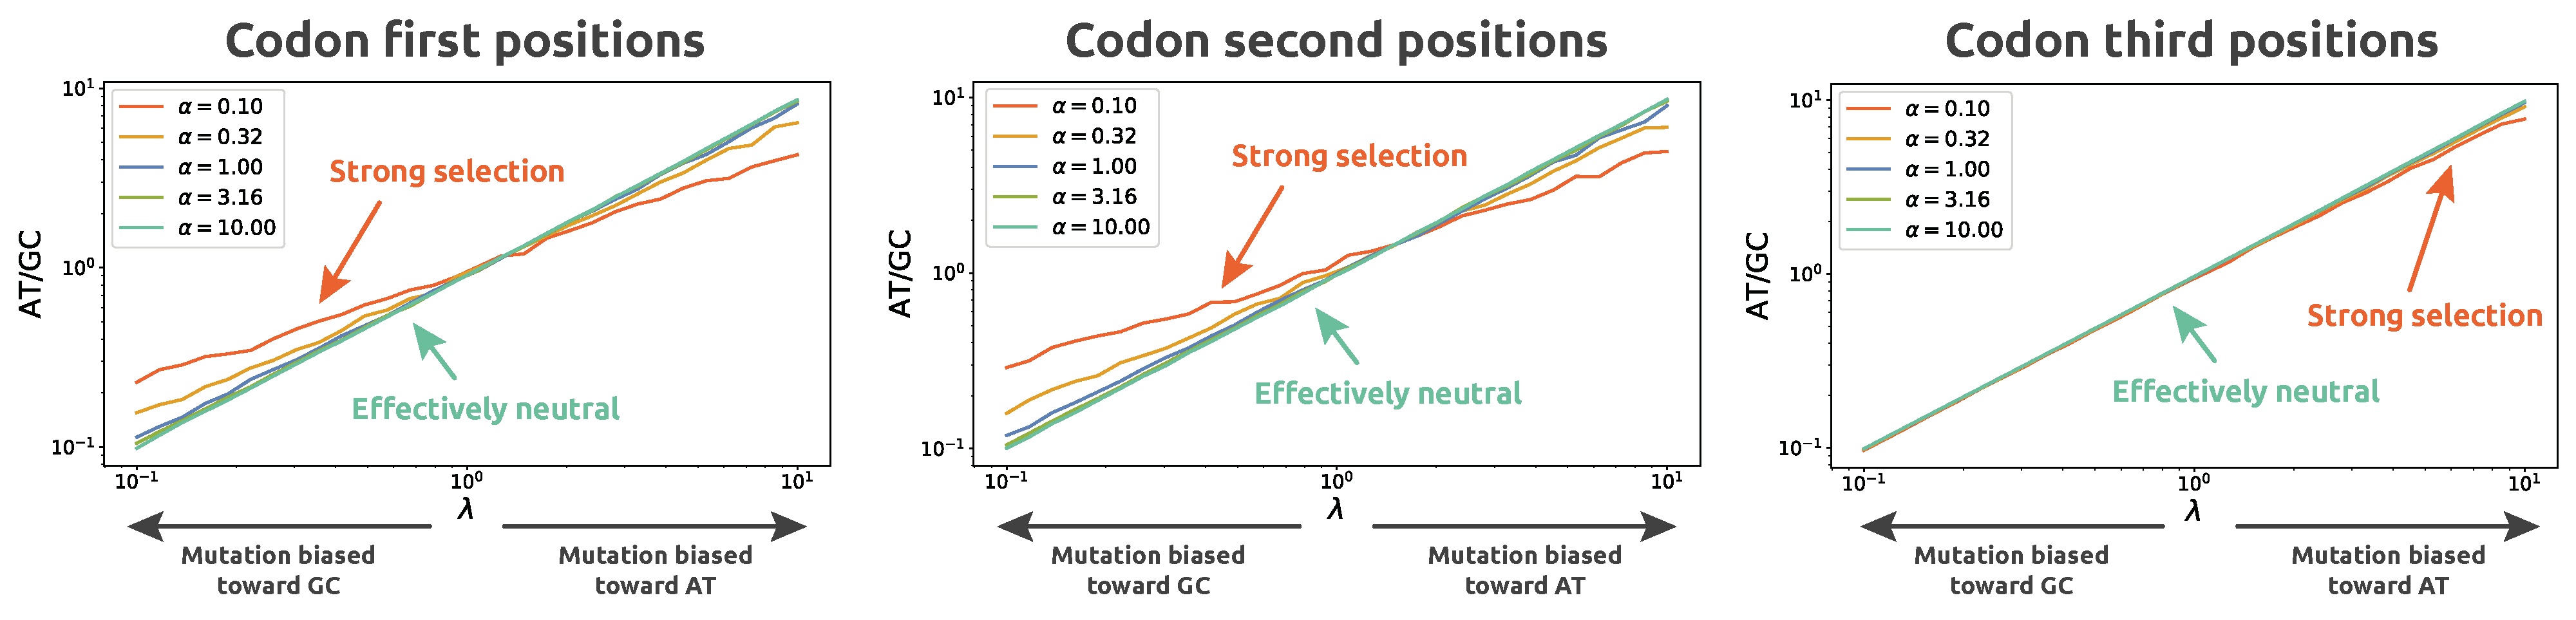
\includegraphics[width=\textwidth] {AT-GC-obs}
    \caption[$\atgc$ composition of the alignment]{
    Observed $\atgc$ composition of the alignment, represented at the different positions of codons (first, second and third), summed over all sites.
    The horizontal axis represents the underlying mutational bias ($\lambda$) of the nucleotide matrix, and the vertical axis represent the observed $\atgc$ of the codon position across the alignment.
    $\atgc$ at the third codon position matches the mutational bias, whereas in contrast first and second positions are less extreme than the underlying bias.
    With increase stringency of selection (decreasing $\alpha$), the observed bias is less and less sensitive to the underlying mutational bias such that selection is balancing the mutational bias.}
    \label{fig-mut-bias:AT-GC-obs}
\end{figure}

Beside the observed mutational bias of the alignment, the diversity of amino acids is an important indicator of the selective constraints that the sequence experiences.
This diversity is quantified by the frequencies of amino acids observed across all taxa in the alignment, summarized through a single statistic, namely entropy of frequencies~\citep{Goldstein2017}, as described in section~\ref{subsec:entropy}.
Entropy can be quantified for a given site of the sequence, and this site-specific entropy can subsequently be averaged over the sequence.
Alternatively, the entropy can be quantified directly on the whole sequence by the observed frequencies of amino acids in the alignment.
These two variants of entropy are computed for alignment under different values of $\alpha$ and $\lambda$, as depicted in figure~\ref{fig-mut-bias:diversity-aa}.
Under stringent selection, only a small number of amino acids are actually permissible any given site resulting in low site-specific entropy.
Yet all amino acids occur at comparable frequencies in the alignment resulting in high sequence entropy. %~\citep{Ramsey2011}.
This analysis highlights how important it is to distinguish between averaged site-specific entropy (left panel) and sequence entropy (right panel).
Moreover, the mutational bias (either toward AT or toward GC) greatly reduces both site-specific and sequence entropy, such that the composition of amino acids is highly dependent on the underlying mutational bias.
This effect is less visible whenever selection is more stringent (decreasing $\alpha$), but can still be observed even for stringent selection.

\begin{figure}[H]
    \centering
    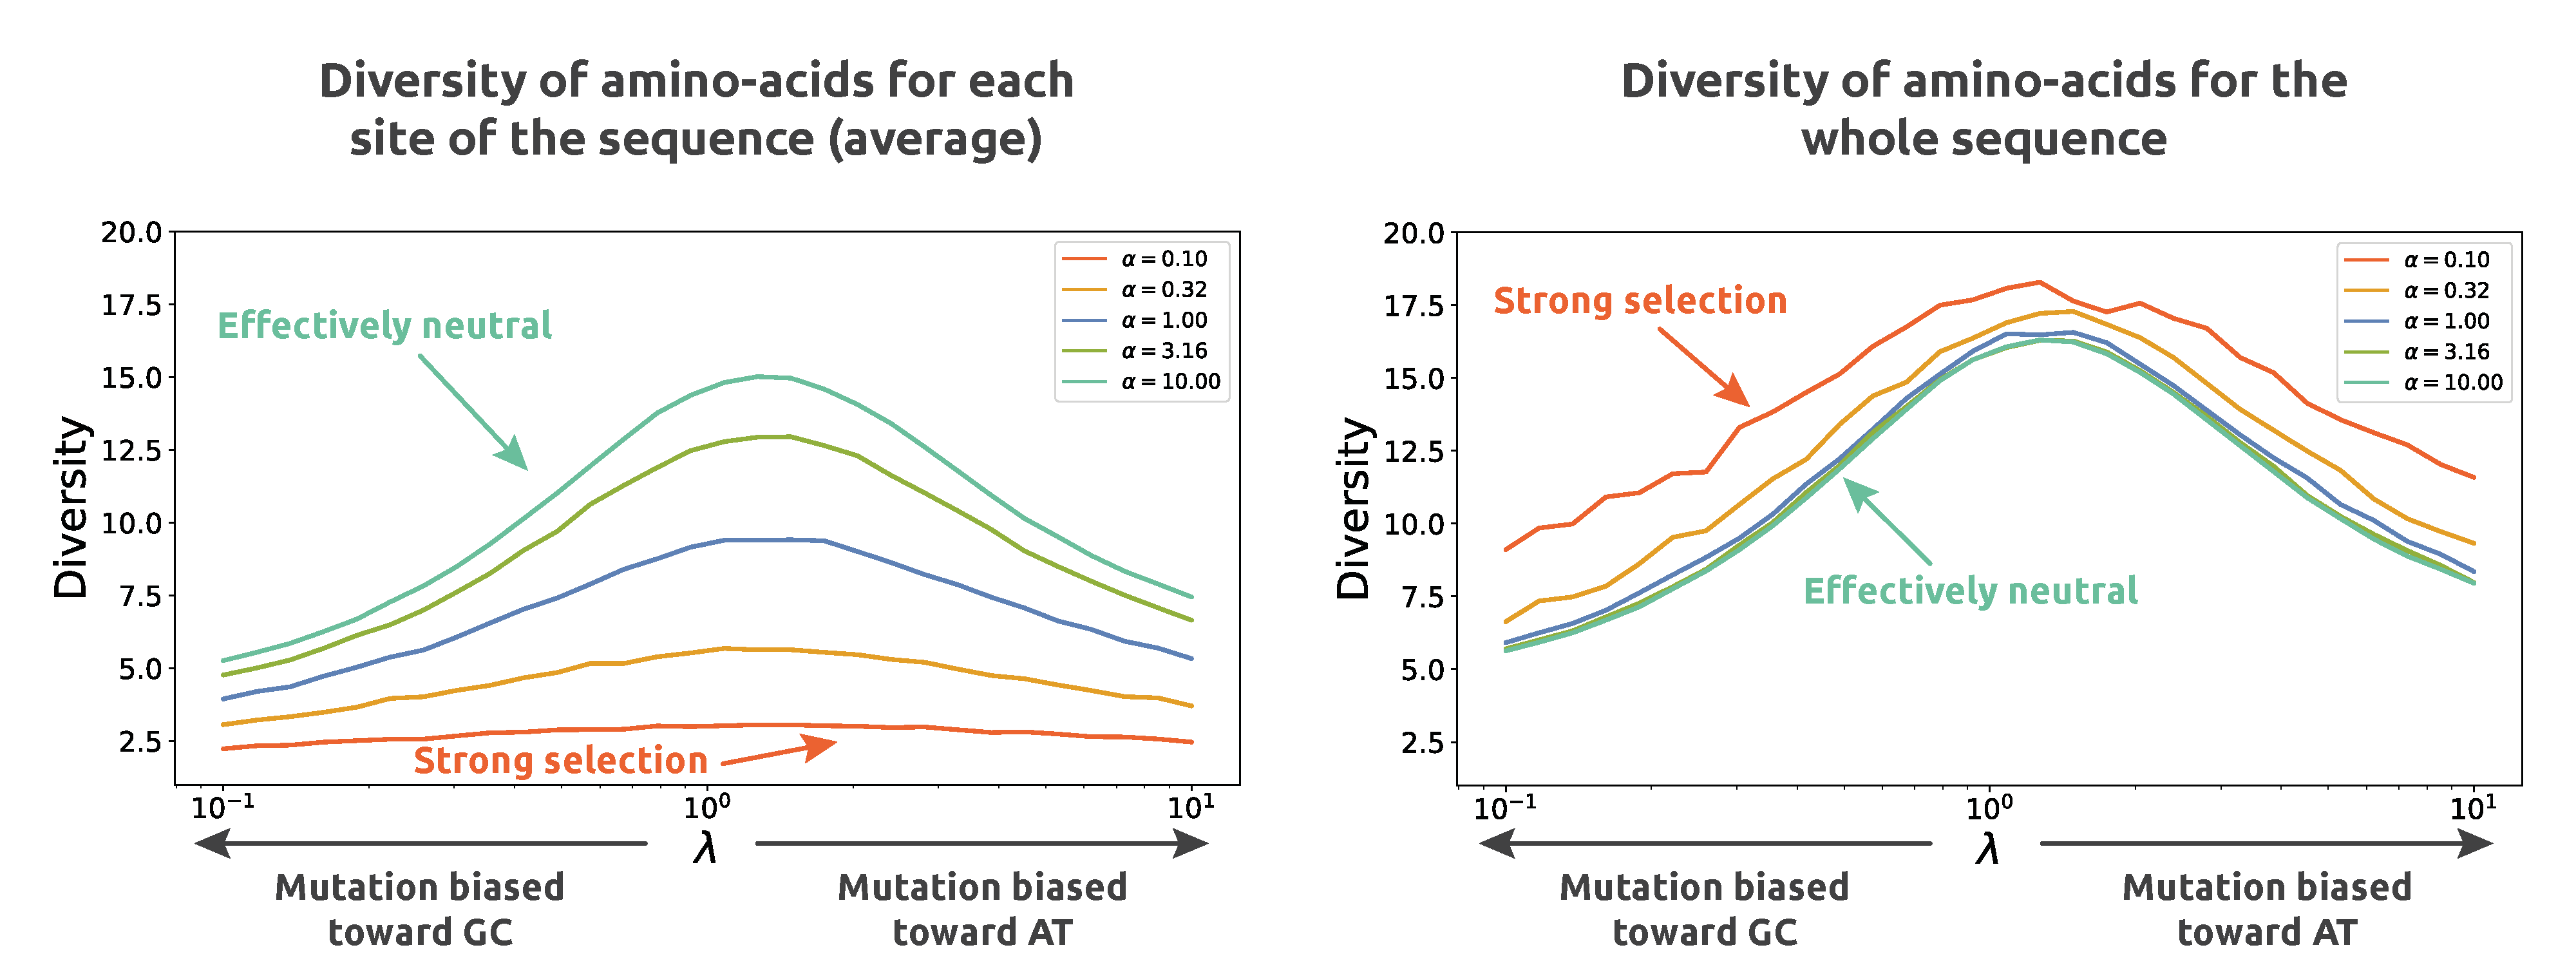
\includegraphics[width=\textwidth] {diversity-aa}
    \caption[Diversity of amino acids]{
    Diversity of amino acids quantified as the entropy of the amino-acid frequencies in the vertical axis, either as site-specific entropy in left panel or as sequence entropy in the right panel.
    Sequence entropy is higher than site-specific entropy, because at any given site only a small number of amino acids are actually permissible.
    From a mutational perspective, entropy decreases with mutational bias toward AT ($\lambda$ in horizontal axis) because mutation bias increases the frequency of AT rich amino acids, while reducing the frequency of GC rich amino acids.
    From a selective perspective, site-specific entropy decreases with stringency of selection (decreasing $\alpha$ represented by 5 different solid lines) because at given site only a few amino acids are permitted.
    Conversely, because site-specific fitness profiles are randomly drawn, each site has different permitted amino acid, increasing the sequence entropy as the stringency of selection increases.
    Moreover, under stringent selection, entropy is less sensitive to mutational bias.}
    \label{fig-mut-bias:diversity-aa}
\end{figure}

%Evolutionary rate, which measures the rate at which mutations at individual sites arise and go to fixation, is governed by the amino acid distribution of individual sites, not the average distribution over a broad class of sites.
%The substitution rate (e.g., Grishin, Wolf \& Koonin, 2000).
%These two measures of evolutionary variability are considered to be essentially equivalent~\citep{Halpern1998}, though they are differently influenced by the mutational process~\citep{Santos2018}.

Because the sequences are not independent but related together by a specie tree, entropy obtained from the observed alignment does not converge to entropy of the substitution process.
Moreover, this measure of stringency of selection does not relate directly to the fixation probability of proposed mutations.
Instead, the mean scaled fixation probability of non-synonymous mutations ($\avgpfix$), which measures the rate at which mutations arise and go to fixation relatively to neutral mutation, is an aggregate parameter measuring the overall strength of selection throughout the process.
Moreover, $\avgpfix$ can be quantified from the substitutions recorded along the simulation (see section~\ref{subsec:fixation-bias}).
As expected, $\avgpfix$ depends strongly on the stringency of selection ($\alpha$), but, however, depends weakly on the mutational bias ($\lambda$), as depicted in left panel of figure~\ref{fig-mut-bias:omega-WS}).
Mean scaled fixation probability ($\avgpfix$) concerns all non-synonymous mutations, but we can consider only the subset of non-synonymous mutations from weak nucleotides (A or T) to strong nucleotides (G or C), called $\avgpfix_{AT \rightarrow GC}$.
With increased mutational bias toward AT ($\alpha$), the mean scaled fixation probability toward GC ($\avgpfix_{AT \rightarrow GC}$) increases in response, as seen in the right panel of figure~\ref{fig-mut-bias:omega-WS}.
The effect is stronger whenever the stringency of selection increases ($\alpha$ decreases).
In other words, selection is opposed to mutational bias, which had pushed sites toward less fit amino acids.

\begin{figure}[H]
    \centering
    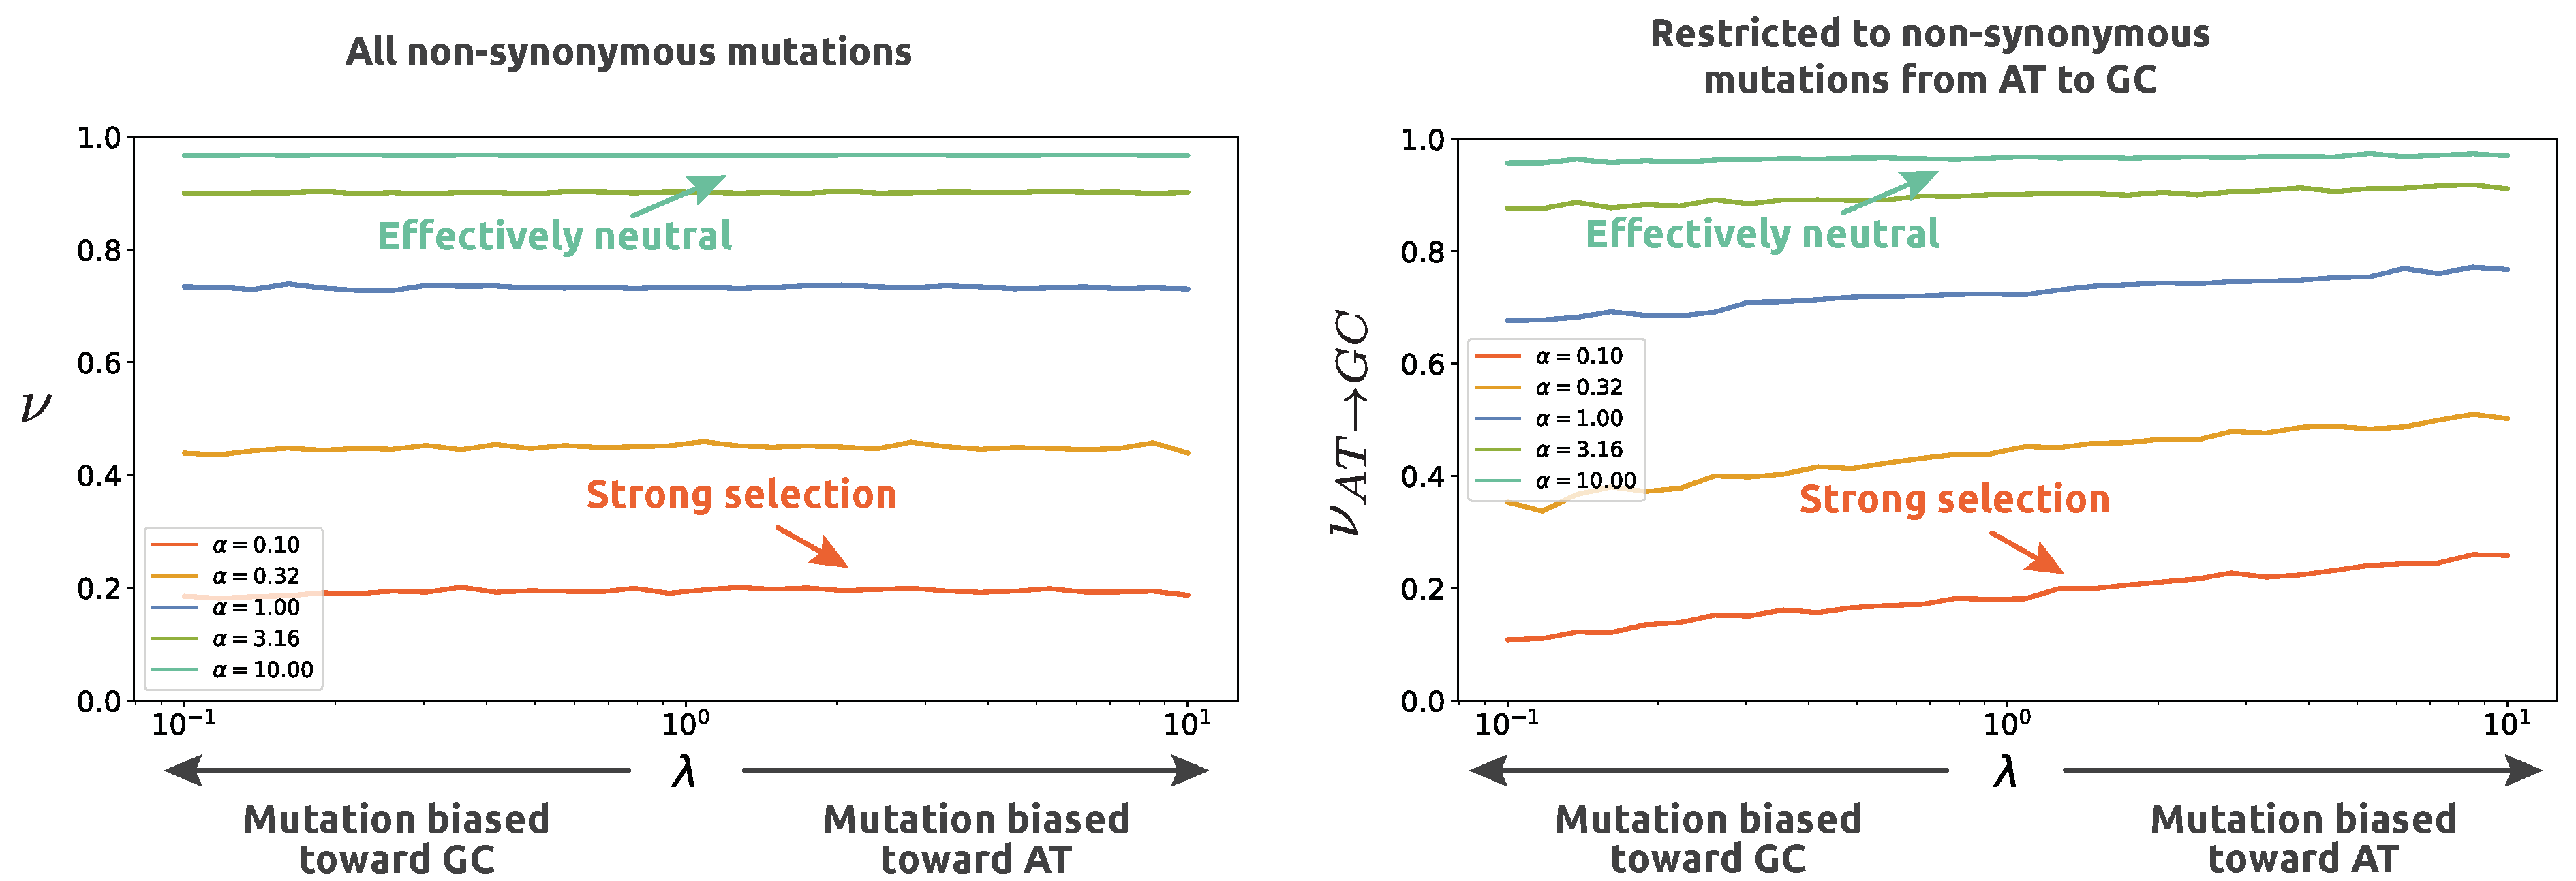
\includegraphics[width=\textwidth] {omega-AT-to-GC}
    \caption[Mean scaled fixation probability as a function of the parameters]{
    Mean scaled fixation probability ($\avgpfix$) in vertical axis as a function of mutational bias ($\lambda$) in the horizontal axis, for different stringency of selection ($\alpha$) in coloured solid lines.
    In right panel, $\avgpfix$ of all non-synonymous mutations is always lower than $1$ for simulation under a fixed fitness landscape~\citep{Spielman2015}.
    Expectedly, $\avgpfix$ decrease with the strength of selection (decreasing $\alpha$).
    However, $\avgpfix$ is relatively unaffected by the strength of the mutational bias.
    In right panel, the mean scaled fixation probability of non-synonymous mutations restricted to mutations from weak nucleotides (AT) to strong nucleotides (GC), $\avgpfix_{AT \rightarrow GC}$ is represented in the vertical axis.
    Mutation biased from GC to AT leads to a mean scaled fixation probability in the opposite direction.
    More generally, mutation bias is balanced by selection, even more strongly that the stringency of selection is strong.
    This is confounding factor with gBGC.}
    \label{fig-mut-bias:omega-WS}
\end{figure}

\subsection{Parameter inference on simulated data}

From an alignment protein-coding \acrshort{DNA} sequences, without knowing the specific history of substitutions, models of inference can estimate the mutational bias ($\lambda$) and mean scaled fixation probability ($\avgpfix$).
Once estimated from the alignment, the biases can be compared to the known value used during the simulation (see figure~\ref{fig-mut-bias:pipeline}).
Two models of inference are proposed, the first is based on Muse \& Gaut formalism, and the second based on a tensor of mean scaled fixation probabilities.

\begin{figure}[H]
    \centering
    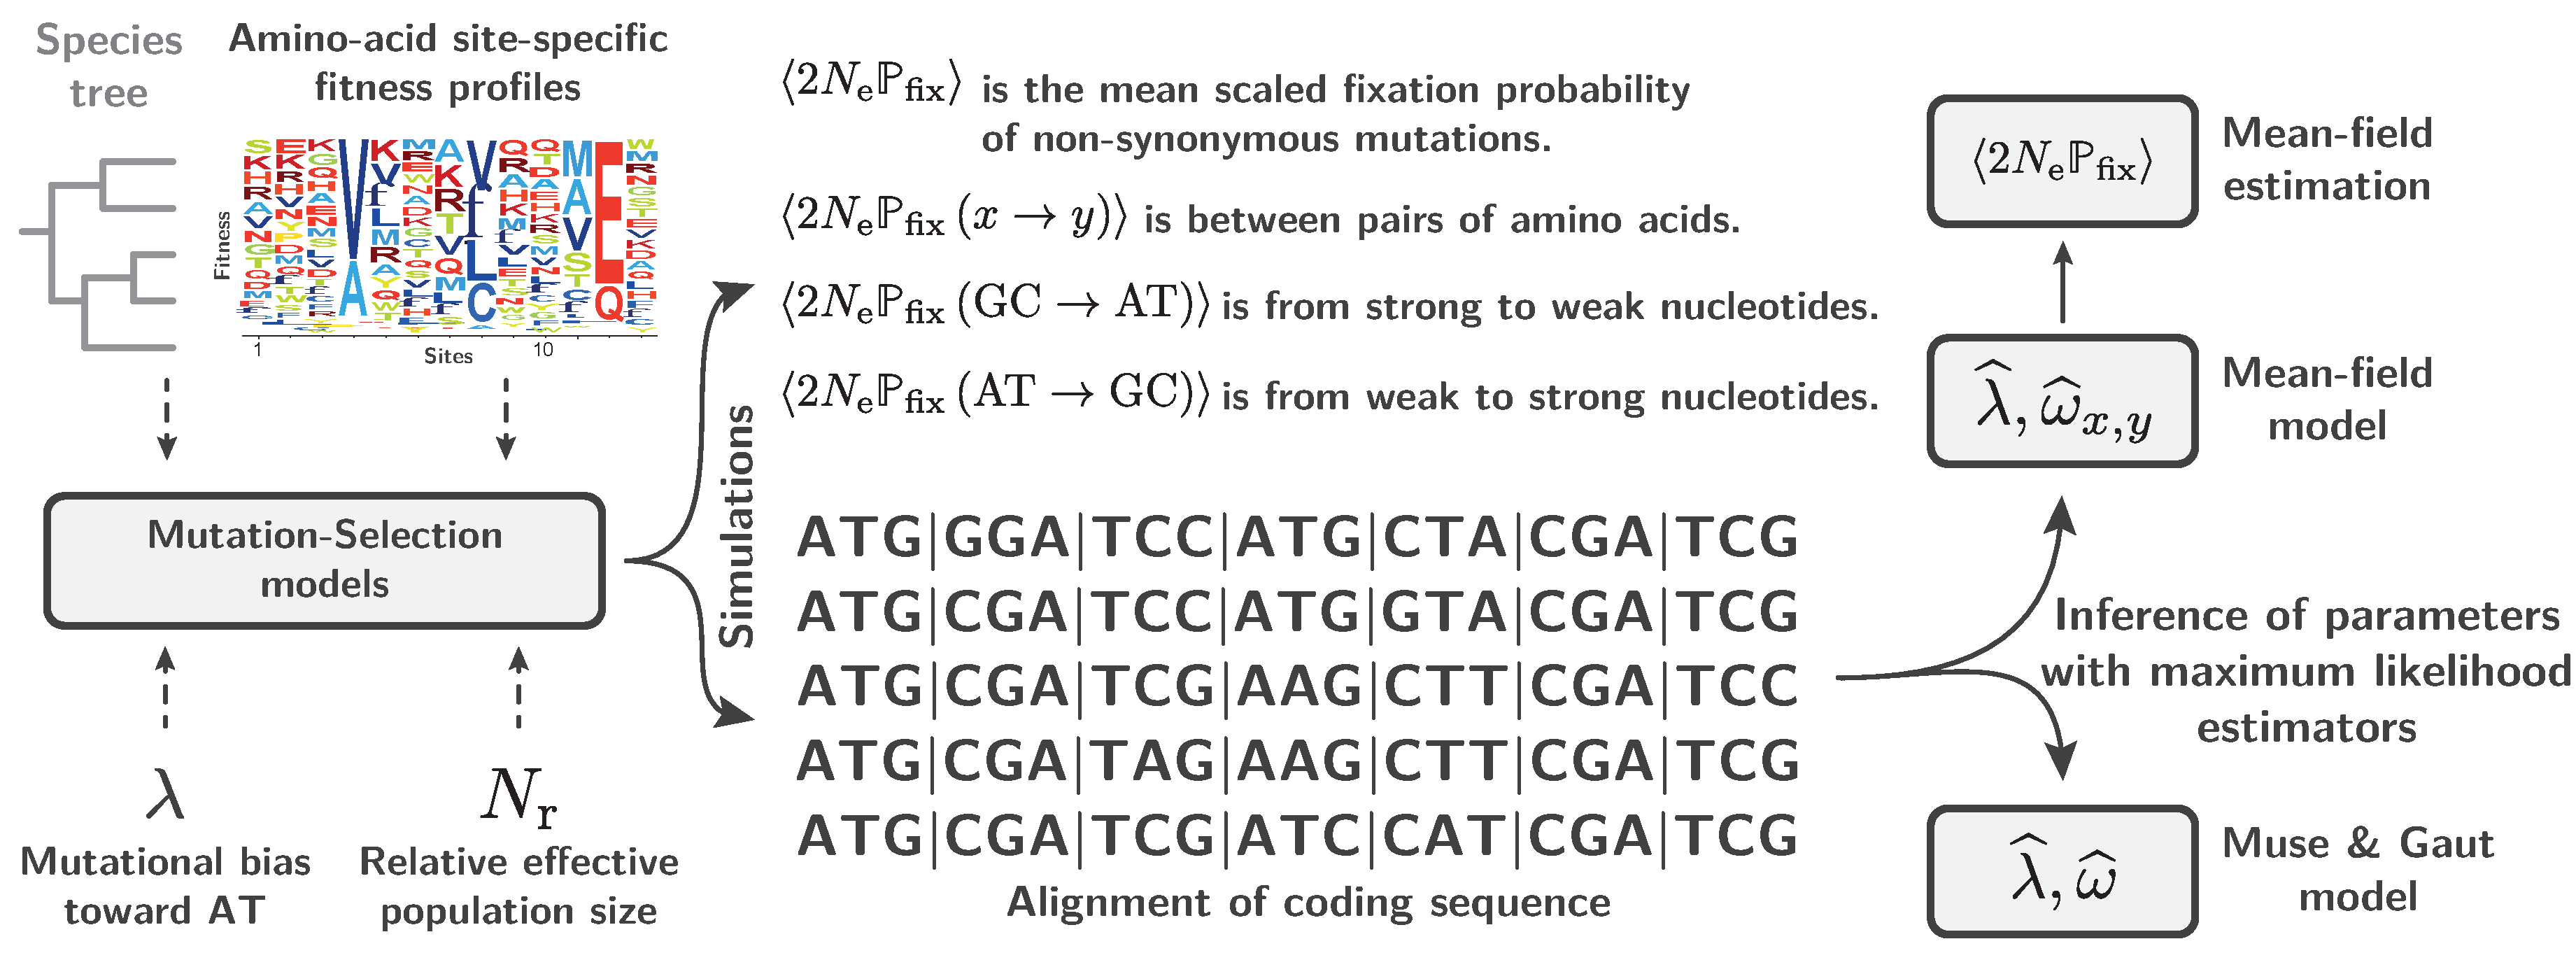
\includegraphics[width=\textwidth, page=1] {pipeline}
    \caption[Inferred value compared to known value]{
    Inferred value compared to underlying value used during the simulation.
    The different parameterization of the inference model can result in different estimates of mutation and mean scaled fixation probability.
    The main goal is to derive model of inference that can reliably estimate the biases.
    Two models of inference are proposed, the first is based on Muse \& Gaut formalism, and the second based on a tensor of mean scaled fixation probabilities.}
    \label{fig-mut-bias:pipeline}
\end{figure}

\subsubsection{$\omega$ as a scalar: the Muse \& Gaut formalism}

The $61$-by-$61$ codon substitution matrix of \citet{Muse1994} is defined entirely by the GTR mutation matrix ($\Mutmatrix$), a single parameter of selective strength $\omega$, and the genetic code:
\begin{equation}
    \begin{dcases}
        \submatrix_{\itoj} & = 0 \text{ if codons $\ci$ and $\cj$ are not one mutation away} \\
        \submatrix_{\itoj} & = \mutmatrix_{\nucitoj} \text{ if codons $\ci$ and $\cj$ are synonymous} \\
        \submatrix_{\itoj} & = \omega \mutmatrix_{\nucitoj} \text{ if codons $\ci$ and $\cj$ are non-synonymous} \\
        \submatrix_{\ci, \ci} & = - \sum\limits_{\cj \neq \ci} \submatrix_{\itoj},
    \end{dcases}
    \label{eq:codon-muse-gaut}
\end{equation}
where $\nucitoj$ denotes the nucleotide change between codon $\ci$ and codon $\cj$.
Phenomenological codon models are not designed to tease out mutational bias, but firstly to estimate the global strength of selection.
From the maximum likelihood estimates of the $4 \times 4$ GTR mutation matrix ($\widehat{\Mutmatrix}$), we can estimate of the mutational bias toward $\mathrm{AT}$ $\left({\widehat{\lambda}_{\text{MG}}} \right)$.
As shown in the left panel of figure \ref{fig-mut-bias:inference}, estimate of the mutational bias is halfway between observed bias of the alignment and the true value used during the simulation.
As a result, this model cannot reliably infer the mutational bias, and is doing a compromise between estimating the selection coefficients and mutational bias.
We can also estimate the parameter ${\widehat{\omega}_{\text{MG}}}$, which is close to the underlying mean scaled fixation probability $\avgpfix$ of the simulation, with an error rate of 1.8\%.

\subsubsection{$\omega$ as a tensor: mean-field derivation}

Alternatively, gene-wide parameters of fixation should attempt to capture and aggregate site-specific parameterization of evolution.
As a result, projecting site-specific processes into a gene-wise process can be seen as a mean-field approximation, accounting for mean scaled fixation probability between amino acids, even though done at the level of the gene.

\begin{align}
    \langle \avgpfix \rangle_{\itoj} & \simeq \langle \avgpfix_{\itoj} \rangle \\
    & = \dfrac{ \langle \pi_{\ci} 2\Ne P_{\mathrm{fix}}(\itoj) \rangle }{ \langle \pi_{\ci} \rangle } \\
    & = \dfrac{ \sum\limits_{\site}  \pi_{\ci}\dfrac{\Fitj\siteexp - \Fiti\siteexp}{1 - \e^{\Fiti\siteexp - \Fitj\siteexp}} }{ \sum\limits_{\site} \pi_{\ci} }
\end{align}

Under projected mutation-selection model, the $61$-by-$61$ codon substitution matrix of codon is defined entirely by the mutation matrix ($\Mutmatrix$), the mean scaled fixation probability between all pairs of amino acids $\omega_{\aai, \aaj}$ and the genetic code:
\begin{equation}
    \begin{dcases}
        \submatrix_{\itoj} & = 0 \text{ if $\ci$ and $\cj$ are non neighbors}, \\
        \submatrix_{\itoj} & = \mu_{\itoj} \text{ if $\ci$ and $\cj$ are synonymous}, \\
        \submatrix_{\itoj} & = \mu_{\itoj} \omega_{\aai, \aaj} \text{ if $\ci$ and $\cj$ are non-synonymous}, \\
        \submatrix_{\ci, \ci} & = - \sum\limits_{\cj \neq \ci} \submatrix_{\itoj}.
    \end{dcases}
    \label{eq:codon-mean-field}
\end{equation}
For $20$ amino acids, the total number of pairs of amino acid is $190$.
However, because of the structure of the genetic code, they are $75$ pairs one nucleotide away, because some amino acids are not directly accessible through a single non-synonymous mutation.
As a result, the number of parameters necessary to determine all mean scaled fixation probability ($\omega_{\aai, \aaj}$) in both directions is $150$.
However, under the assumption of a reversible process, the number of parameters can be reduced to $75$ parameters of exchangeabilities ($\beta_{\aai, \aaj}$) and $20$ parameters of stationary distribution ($\epsilon_{\aai}$).
\begin{align}
    \omega_{\aai, \aaj} = \epsilon_{\aaj} \beta_{\aai, \aaj}, \\
    \text{ where } \beta_{\aai, \aaj} = \beta_{\aaj, \aai}.
\end{align}
The process is reversible:
\begin{align}
    \epsilon_{\aai} \omega_{\aai, \aaj} & = \epsilon_{\aai} \epsilon_{\aaj} \beta_{\aai, \aaj}, \\
    & = \epsilon_{\aaj} \omega_{\aaj, \aai}
\end{align}

From the maximum likelihood estimates of the GTR mutation matrix ($\widehat{\Mutmatrix}$), we can estimate the mutational bias $\left({\widehat{\lambda}_{\text{MF}}} \right)$ as previously.
As shown in the right panel of figure \ref{fig-mut-bias:inference}, estimate of the mutational bias can tease out observed bias of the alignment and true value.
We can also estimate the mean scaled fixation probability of non-synonymous mutations $\left({\widehat{\omega}_{\text{MF}}} \right)$ (see section~\ref{sec-mut-bias:mean-field-omega}) which is a compound parameter of the mutation matrix and the mean scaled fixation probability in the different direction.
Error of the estimated non-synonymous mean scaled fixation probability is 3.0\%.

\begin{figure}[H]
    \centering
    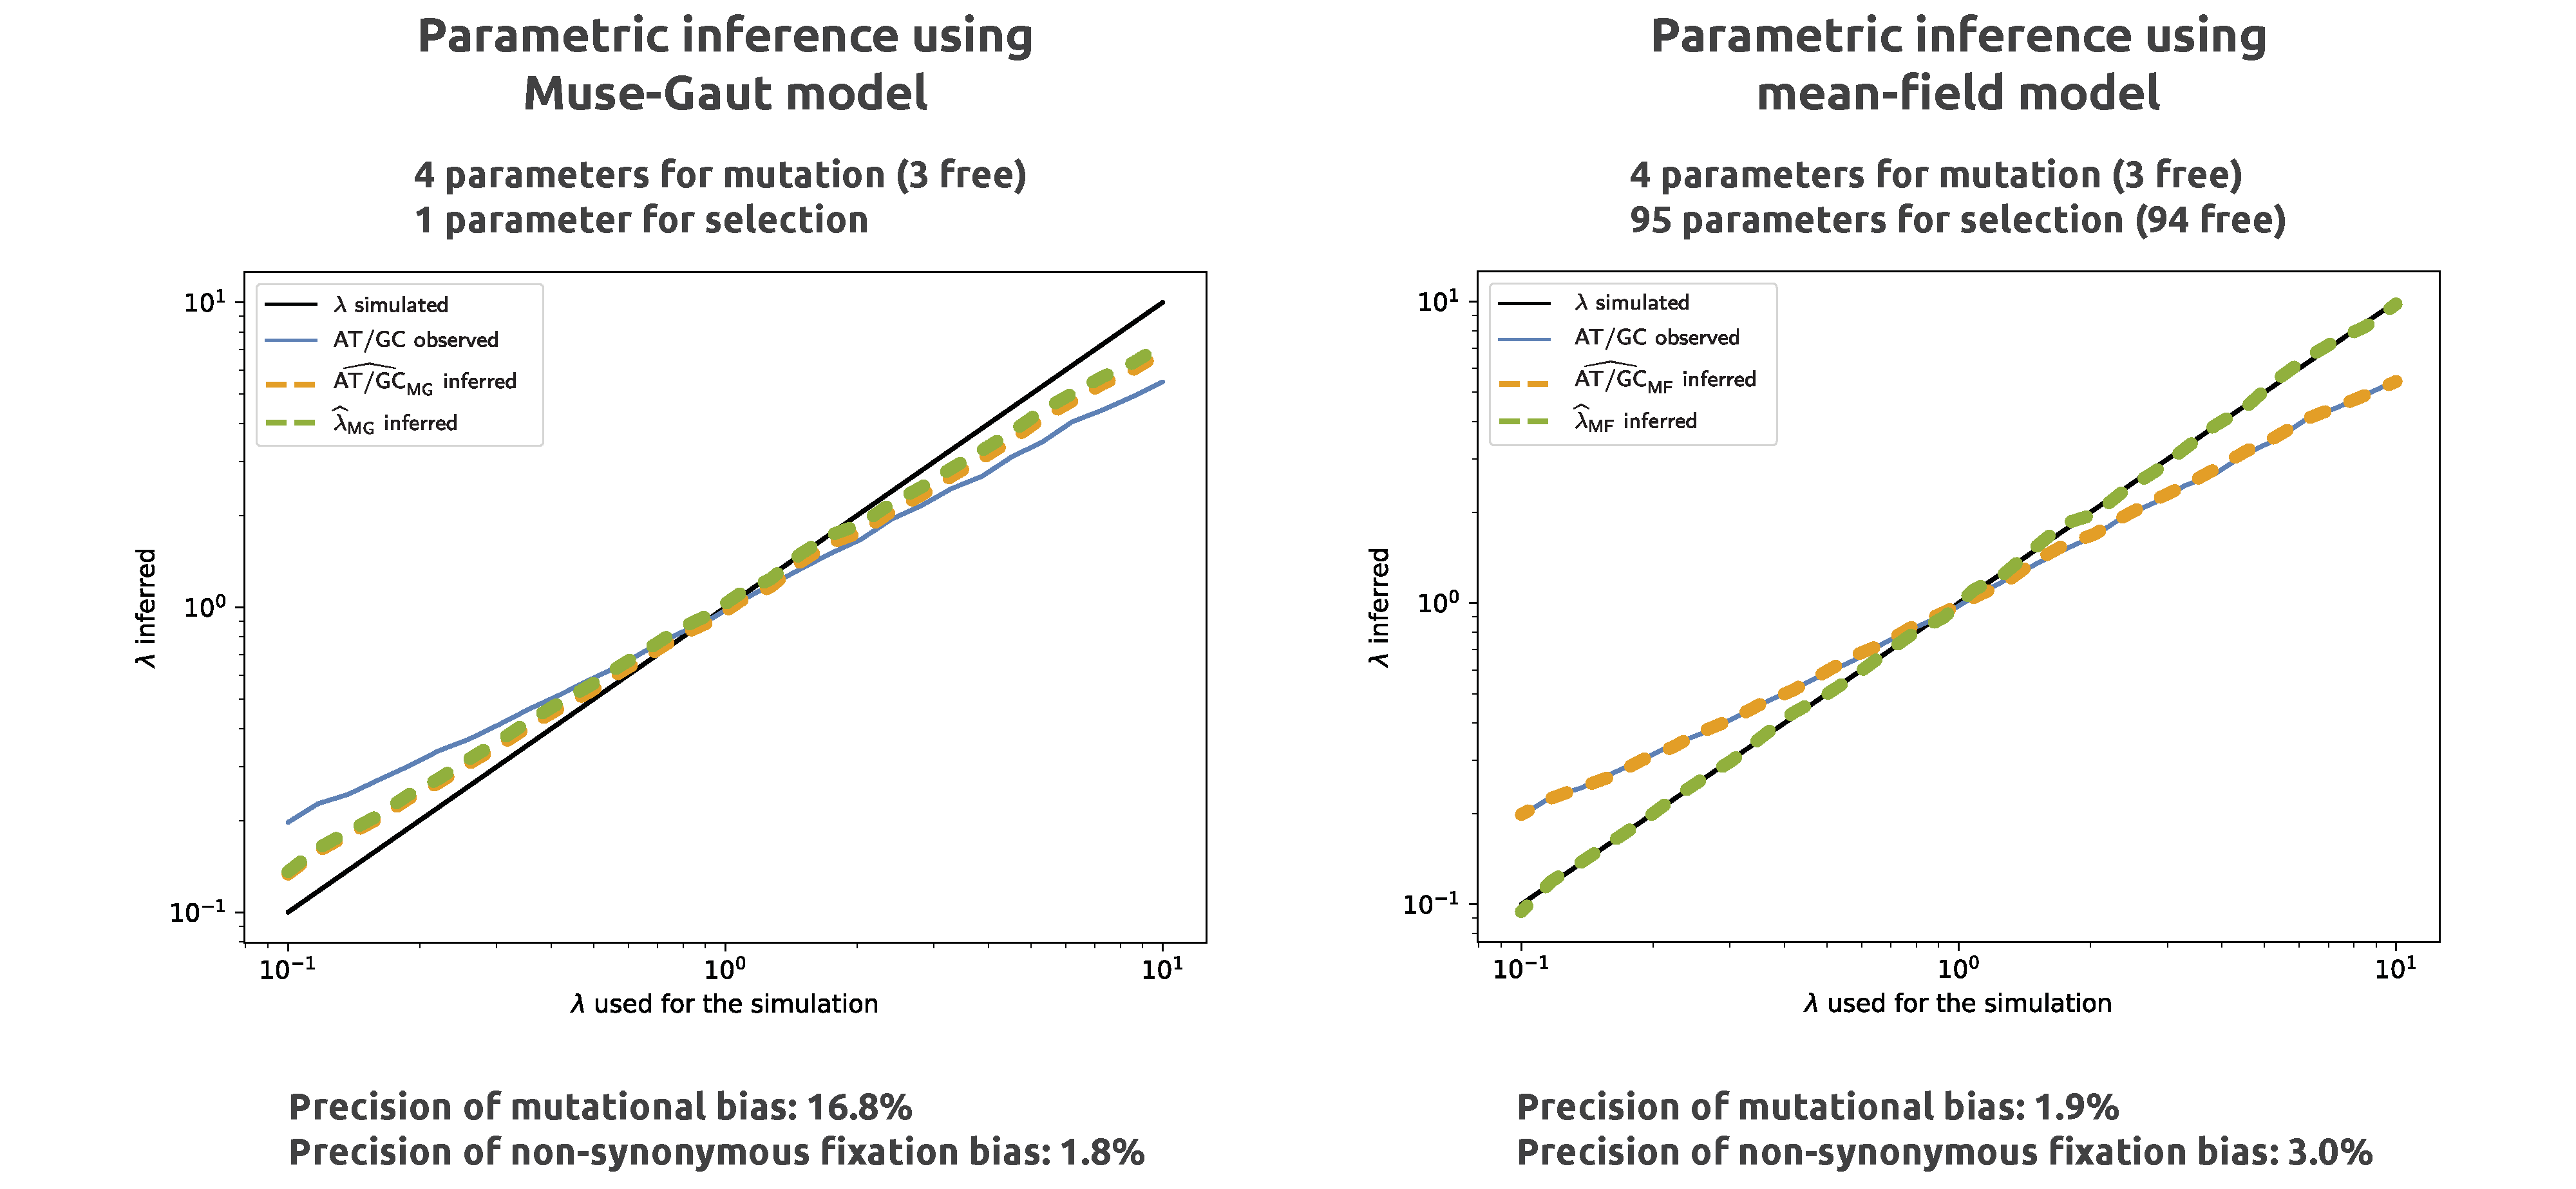
\includegraphics[width=\textwidth] {Simulation-vs-Inference}
    \caption[Estimation of mutation and mean scaled fixation probability]{
    Estimation of mutational bias.
    Modelling a single mean scaled fixation probability leads to skewed estimation of mutation bias.
    Modelling multiple mean scaled fixation probability leads to precise estimation of mutation bias}
    \label{fig-mut-bias:inference}
\end{figure}

\subsection{Estimation of empirical sequence data}

The two models of inference (classical Muse \& Gaut and mean-field) can be applied to empirical alignment.
Also, in empirical data we observed that the mean scaled fixation probability between weak and strong nucleotide is not equal, and is opposite of the nucleotide bias (see table~\ref{table-mut-bias:estimation}).

\begin{table}[H]
    \centering
    \noindent\adjustbox{max width=\textwidth}{%
    \begin{tabu}{|c||c|c|}
        \hline
        \textbf{Estimated parameter} & Nucleoprotein & Lactamase \\
        \hline \textbf{$\atgc$ of the alignment} & 1.15 & 0.79 \\
        \hline \textbf{Muse-Gaut mutational bias $\left({\widehat{\lambda}_{\text{MG}}} \right)$ } & 1.39 & 0.85 \\
        \hline \textbf{Mean-field mutational bias $\left({\widehat{\lambda}_{\text{MF}}} \right)$} & 1.64 & 0.68 \\
        \hline \textbf{Mean-field fixation ratio from AT to GC $\left(\widehat{\omega}_{\textbf{AT} \rightarrow \textbf{GC}}\right)$} & 0.14 & 0.31 \\
        \hline \textbf{Mean-field fixation ratio from GC to AT $\left(\widehat{\omega}_{\textbf{GC} \rightarrow \textbf{AT}}\right)$} & 0.10 & 0.44 \\
        \hline
    \end{tabu}}
    \caption[Estimated parameters]{
    Nucleoprotein alignment of 498 amino acids available for 180 species (left column).
    Lactamase alignment of 263 amino acids available for 85 species (right column).
    }
    \label{table-mut-bias:estimation}
\end{table}


\section{Discussion}

The observed composition DNA is the result of the interplay between mutation and selection, such that observed mutational bias in the alignment is different to the underlying mutational bias.
In protein-coding DNA sequence, the nucleic composition result in the subtle interplay between mutation at the nucleic level and selection at the protein level.
For example, mutational bias toward AT is balanced by selection in the opposite direction toward GC, potentially a confounding effect with gBGC.

Unfortunately, parametric codon models developed to estimate the rate of evolution on amino acids use the observed mutational bias at the protein level, discarding the effect of selection.
We show that even if the mutational process is misspecified, parametric codon models are able to estimate reliably the rate of evolution acting on amino acids.
However, such parametric codon models are inherently misspecified to untangle mutation and selection, and they don't estimate the mutational process reliably.
Reliable inference of mutational bias thus requires to model selection in different directions.

In this work we seek to find the simplest parametric codon model able to correctly tease apart mutation rates on one hand, and net mean fixation probabilities without having to explicitly model the underlying fitness landscape.
In order to derive a codon model along those lines, our strategy is to first assume a true site-specific evolutionary process, following the mutation-selection formalism.
For the sake of simplicity and illustration, we assume a site-specific, fixed fitness landscape.
Then, we derive the mean substitution process implied across all sites by this site-specific mechanistic model.
This mean-field $61$x$61$ substitution matrix is expressed in terms of mutation rates and average fixation probabilities.
Finally, we identify average fixation probabilities appearing in this expression with the $\omega$ tensor we are looking for.
What we show is that we should in fact invoke as many distinct $\omega$ parameters as there are pairs of amino acids that are nearest neighbours in the genetic code.
There are reversibility conditions, reducing the dimensionality and allowing for a GTR-like parameterization of this tensor ($95$ parameters for selection).

Our model
Inferring parameters on simulated alignments, we show that the model correctly estimates the mutation rates.
Our mean-field parametric model use gene-wise parameters of mean scaled fixation probabilities, and even though the underlying selective landscape is site-specific, such approximation can nonetheless be used to disentangle mutation and selection.

Our model infers gBGC
Applied to empirical data, we observe that selection toward GC absorbed in the $\dnds$ is also

\section{Materials \& Methods}

\subsection{Simulation model}
\label{sec-mut-bias:simu}
We seek to simulate the evolution of protein-coding sequences along a specie tree.
Starting with one sequence at the root of the tree, the sequences evolves independently along the different branches of the tree by point substitutions, until they reach the leaves.
At the end of the simulation, we get one sequence for each leaf of the tree, meaning one sequence per specie.
Such evolutionary process is an idealized version of the reality, in the sense that the whole heterogeneity of sequences in the population is wiped away, with only one sequence representing the whole population.
For a protein-coding \acrshort{DNA} sequence, a substitution is modelled as the product of mutation at the nucleotide level, and selection at the amino-acid level.
On one hand, the mutation rate between nucleotides as assumed to be shared by all sites of the sequences.
On the other hand, the selection for amino acids is assumed to be varying along the sequences.
During the simulation, from a given sequence, the substitution rate toward all possible mutant (one nucleotide change) is computed and the next substitution at the waiting time until such event is obtained by Gillespie algorithm.

\subsubsection{Mutational bias at the nucleotide level}
\label{sec-mut-bias:mut-matrix}
The mutation rate between nucleotides is always proportional to $\mu$.
Moreover, mutations from any nucleotide to another weak nucleotide is increased by the factor $\lambda$ compared with mutations to another strong nucleotide.
The rate at which a nucleotide doesn't change is given such as the sum of all rates is zero.
The mutation rate matrix is:
\begin{equation}
    \label{nucMatrix}
    \Mutmatrix =
    \begin{pmatrix}
    {-\mu(2 + \lambda)}
        & {\mu} & {\mu} & {\mu \lambda} \\
        {\mu \lambda} & {-\mu(1 + 2\lambda)} & {\mu} & {\mu \lambda} \\
        {\mu \lambda} & {\mu} & {-\mu(1 + 2\lambda)} & {\mu \lambda} \\
        {\mu \lambda} & {\mu} & {\mu} & {-\mu(2 + \lambda)}
    \end{pmatrix}.
\end{equation}
The stationary distribution $ \Subequi$ must be annihilated by the mutation matrix $\Mutmatrix$, which gives the stationary distribution:
\begin{align}
    \Mutequi \Mutmatrix & = 0, \\
    \iff \Mutequi & = \left( \dfrac{\lambda}{2+2\lambda}, \dfrac{1}{2+2\lambda}, \dfrac{1}{2+2\lambda}, \dfrac{\lambda}{2+2\lambda} \right).
    \label{nucStationarity}
\end{align}
The process is reversible and fulfils detailed balance conditions for any pair of different nucleotides:
\begin{align}
    \mutequi_a \mutmatrix_{a, b} =\mutequi_b \mutmatrix_{b, a}.
    \label{nucMutBalance}
\end{align}
It is important to note that ratio of weak over strong nucleotides frequency at stationarity is equal to $\lambda$:
\begin{align}
    \label{lambda}
    \dfrac{ \mutequi_A + \mutequi_T }{ \mutequi_C + \mutequi_G }
    & = \dfrac{ \lambda ( 2 + 2 \lambda)^{-1} + \lambda ( 2 + 2 \lambda)^{-1}}{ ( 2 + 2 \lambda)^{-1} + ( 2 + 2 \lambda)^{-1}}, \ \textrm{from eq.~\ref{nucStationarity},}\\
    & = \lambda.
\end{align}

\subsubsection{Selection at the amino-acid level}
\label{sec-mut-bias:aa-selection}
The mutation rate between a pair of codons is given by the underlying mutation rates between nucleotides.
However the rate mutation rate is null if the pair of codons differs by more than one nucleotide:
To note, the substitution rate between codons would be equal to the mutation rate if codons are selectively neutral.
However, we subsequently take into the selection acting on codon by modelling it at the amino-acid level, where each amino acid $\aai$ encoded by codons $\ci $are given a fitness ($\Fiti$).
By modelling fitness at the amino-acid level, we assume that all codons encoding for one particular amino acid are selectively neutral.
In this modelling framework, the genetic code is of particular importance since the number of codons encoding for a particular amino acid varies greatly.
As an example, tryptophan is encoded by one codon, while leucine is encoded by 6 codons.
Intuitively, this variation makes the mutation bias more effective in codons encoding for the same amino acids, since there are more mutations possible that are selectively neutral (same amino acid).
While the other hand, the mutation bias is more constrained if the amino acid is encoded by a few codons since there are only a few selectively neutral mutations.\\

To take into account the heterogeneity of selection between different sites of the protein, we assume that each site $\site$ of the sequence is evolving under a different fitness landscape ($\Fiti\siteexp$).
At one particular site, under a static fitness landscape, the substitution rate between codons is given by the product of the mutation rate and the probability of fixation:
\begin{equation}
    \begin{dcases}
        \submatrix_{\itoj} & = 0 \text{ if $\ci$ and $\cj$ are non neighbors} \\
        \submatrix_{\itoj} & = \mu_{\itoj} \text{ if $\ci$ and $\cj$ are synonymous} \\
        \submatrix_{\itoj} & = \mu_{\itoj} \dfrac{\Fitj - \Fiti}{1 - \e^{\Fiti - \Fitj} } \text{ if $\ci$ and $\cj$ are non-synonymous} \\
        \submatrix_{\ci, \ci} & = - \sum\limits_{\cj \neq \ci} \submatrix_{\itoj}
    \end{dcases}
    \label{codonSubRates}
\end{equation}
At the root the tree, the sequence is obtained by sampling from the equilibrium stationary distribution
The stationary distribution $\Subequi$ must be annihilated by the mutation matrix $\Submatrix$, which gives the stationary distribution at site $\site$:
\begin{align}
    \Subequi\siteexp \bm{Q}\siteexp
    & = 0 ,\\
    \iff \subequi_{\ci}\siteexp
    & = \mathcal{Z}\siteexp \lambda^{\nbrWeak_{\ci}} \e^{\Fiti\siteexp},\\
    & \mathrm{ where } \ \mathcal{Z}\siteexp = \left( \sum\limits_{\cj=1}^{61} \lambda^{\nbrWeak_{\cj}} \e^{\Fitj\siteexp} \right)^{-1},
    \label{codonStationarity}
\end{align}
where $\nbrWeak_{\ci}$ is the number of weak nucleotides (A or T) in the codon (between 0 and 3).

Moreover, the substitution process is reversible and fulfils detailed balance conditions at each site $\site$:
\begin{align}
    \subequi_{\ci}\siteexp \submatrix_{\itoj}\siteexp = \subequi_{\cj}\siteexp \submatrix_{\cj, \ci}\siteexp
    \label{codonSubBalance}
\end{align}

\subsection{Observed summary statistics from simulations}
\label{subsec:summary-statistics}

\subsection{Entropy of site and sequence}
\label{subsec:entropy}

For a category $\cat$, the Shannon entropy ($\entropy$) of the fitness profile is defined as:
\begin{equation}
    \entropy\catexp = - \sum\limits_{\aSetAa} \base\catexp_{\aminoacid} \log \left( \base\catexp_{\aminoacid} \right)
\end{equation}
The Shannon entropy measures the flatness of the fitness profile, with a value of $0$ corresponding to a single peak fitness landscape (only one amino acid is present), and a value of $\ln(20)\simeq3$ corresponding to a neutral landscape, where each amino acid has the same fitness.

The Shannon entropy can be averaged over all sites as:
\begin{equation}
    \langle \entropy \rangle = \dfrac{1}{\Nsite}\sum\limits_{\Setsite} \entropy^{\catsite}
\end{equation}

\subsection{Mean scaled fixation probability \texorpdfstring{$\avgpfix$}{φ}}
\label{subsec:fixation-bias}
The mean scaled fixation probability is:
\begin{align}
    \avgpfix & = & = \dfrac{ \sum\limits_{B} Q_{A \to B}}{ \sum\limits_{B} \mu_{A \to B}}
\end{align}

\subsection{Mean scaled fixation probability under the mean-field model}
\label{sec-mut-bias:mean-field-omega}

The mean scaled fixation probability is:
\begin{align}
    \omega_{\text{MF}} & = \dfrac{ \sum\limits_{i} \sigma_{\ci[1]}\sigma_{\ci[2]}\sigma_{\ci[3]} \epsilon_{\aaj} \sum\limits_{j \in \NonSyn_{\ci}} \mu_{\itoj} \epsilon_{\aaj} \beta_{\aai, \aaj} }{\sum\limits_{i} \pi_{i} \sum\limits_{j \in \NonSyn_{\ci} } \mu_{\itoj}}
\end{align}

The mean scaled fixation probability from weak to strong is $\omega_{\textbf{AT} \rightarrow \textbf{GC}}$ is obtained similarly by restricting the sum to one nucleotide mutation only from weak to strong.
Conversely, the mean scaled fixation probability from strong to weak is obtained by restricting one nucleotide mutation only from weak to strong.

\subsection{Inference method with Hyphy}

Maximum likelihood estimation has been performed with the software Hyphy~\citep{Pond2005}.
The python scripts generating the Hyphy batch files (for both Muse \& Gaut and mean-field), as well as scripts to analyse experiments are available at \url{https://github.com/ThibaultLatrille/NucleotideBias}
